\documentclass[border=12]{standalone}

\usepackage{amsmath}
\usepackage{ifthen}
\usepackage{makecell}
\usepackage{pgfmath}
\usepackage{standalone}
\usepackage{stix}
\usepackage{tikz}
\usepackage{tikz-3dplot}
\usepackage{tkz-euclide}
%
%
%
\usetkzobj{all}
\usetikzlibrary{angles}
\usetikzlibrary{arrows.meta}
\usetikzlibrary{arrows}
\usetikzlibrary{automata}
\usetikzlibrary{calc}
\usetikzlibrary{circuits.logic.IEC}
\usetikzlibrary{circuits.logic.US}
\usetikzlibrary{decorations.footprints}
\usetikzlibrary{decorations.markings}
\usetikzlibrary{decorations.pathmorphing}
\usetikzlibrary{decorations.pathreplacing}
\usetikzlibrary{decorations.shapes}
\usetikzlibrary{decorations.text}
\usetikzlibrary{intersections}
\usetikzlibrary{mindmap}
\usetikzlibrary{patterns}
\usetikzlibrary{positioning}
\usetikzlibrary{quotes}
\usetikzlibrary{shadings}
\usetikzlibrary{shadows}
\usetikzlibrary{shapes.callouts}
\usetikzlibrary{shapes.geometric}
\usetikzlibrary{shapes}

%
\definecolor{Grey}{RGB}{76,76,78}
\definecolor{Blue}{RGB}{85,164,224}
\definecolor{Red}{RGB}{225,75,59}
\definecolor{Green}{RGB}{16,158,36}
\definecolor{Orange}{RGB}{243,162,3}
\definecolor{Purple}{RGB}{124,36,231}
\definecolor{Fushia}{RGB}{225,50,162}
%
\definecolor{Grey1}{RGB}{130,130,131}
\definecolor{Blue1}{RGB}{98,170,223}
\definecolor{Red1}{RGB}{236,98,88}
\definecolor{Green1}{RGB}{105,186,108}
\definecolor{Orange1}{RGB}{251,192,79}
\definecolor{Purple1}{RGB}{160,114,235}
\definecolor{Fushia1}{RGB}{237,97,174}


\begin{document}
	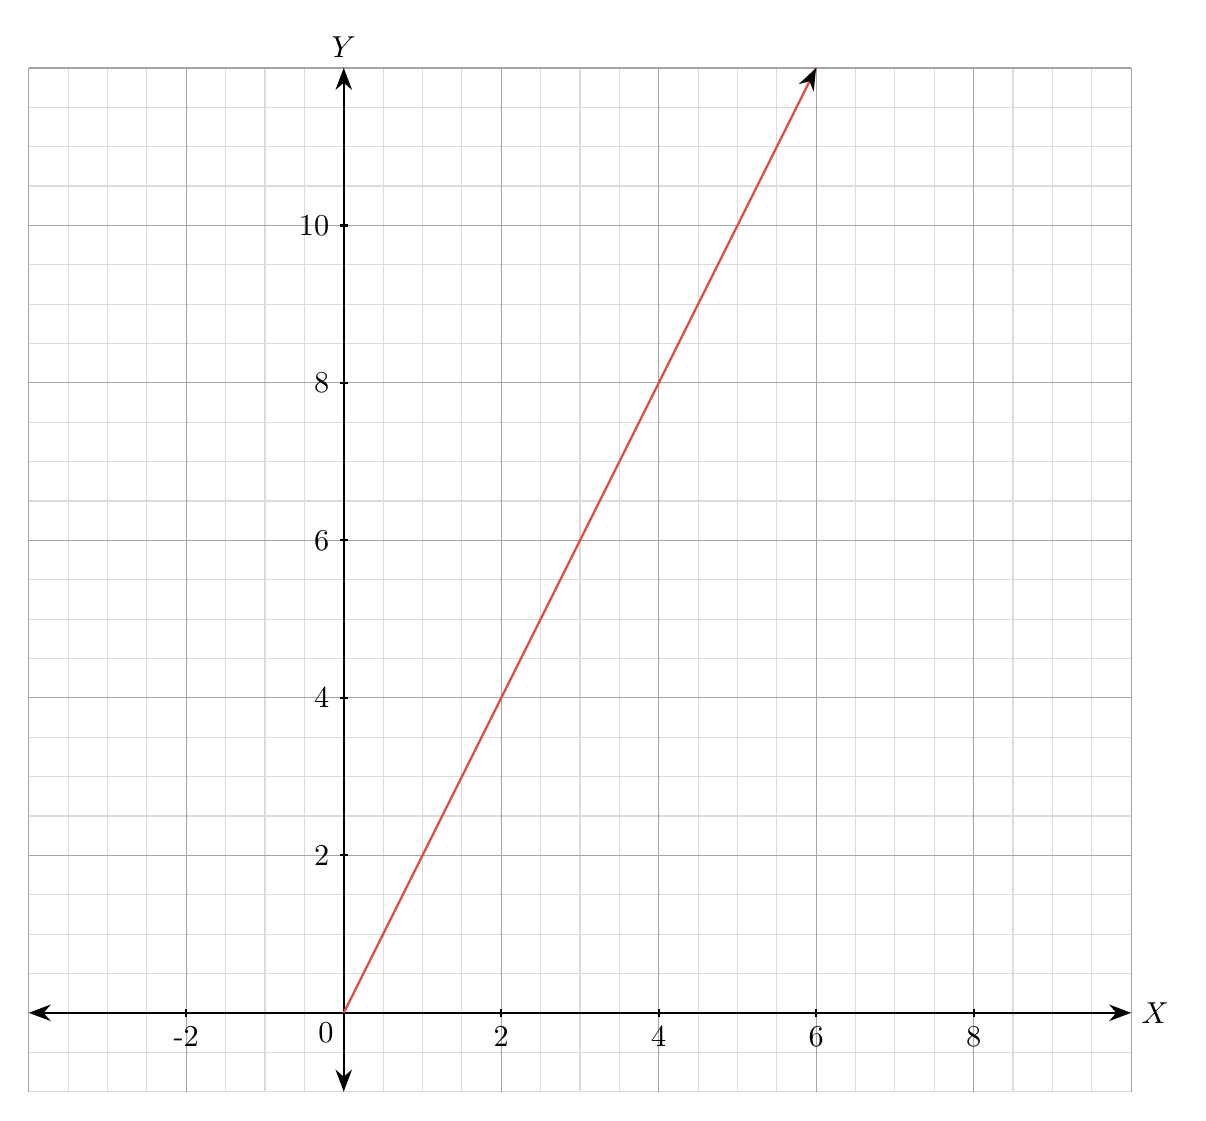
\begin{tikzpicture}
	\begin{scope}[>={Stealth[scale=1.2]}, thick,line join=round, font=\fontsize{11.25}{11.25}\selectfont]
	\pgfgettransformentries{\mya}{\myb}{\myc}{\myd}{\mys}{\myt}
	\pgfmathsetmacro{\preserve}{1/\mya}	

\draw [thin,Grey!20,step=0.5] (-4,-1) grid (10,12);
\draw [thin,Grey!50,step=2]  (-4,-1) grid (10,12);
	
	\foreach \x/\n  in{-2,2,4,6,8}
	\draw (\x,0.35ex)--(\x,-0.35ex)node[anchor=north]{
		\nagwaMathLabel
		{\n}};
	\foreach \y/\m  in{2,4,6,8,10}
	\draw (0.35ex,\y)--(-0.35ex,\y)node[anchor=east] {
		\nagwaMathLabel
		{\m}};
	
\draw [<->] (-4,0)--(10,0) node [anchor=west] {$X$};
\draw [<->] (0,-1)--(0,12) node [anchor=south] {$Y$};
\node [anchor=north east] at (0,0) {$0$};

\draw [Red](0,0)--(6,12);
\path [postaction={decorate, decoration={markings,mark=at position 1 with {\arrow[]{>}}}}](0,0)--(6,12);

	
	\end{scope}
	\end{tikzpicture}
\end{document}